\documentclass[12pt]{article}
% =========================================================================
% SHARED STYLE FILE for 11_Master_Projects reports
% Visual style follows 0_Thesis_Submission/24m0553_AK_Gaurav_Mtech_Report.pdf:
% serif body font, blue hyperlinked TOC/links, ruled section headings,
% IITB-style title page, formal academic report structure.
% =========================================================================

\usepackage[a4paper,margin=1in]{geometry}
\usepackage{xcolor}
\usepackage{graphicx}
\graphicspath{{../images/}}
\usepackage{amsmath,amssymb}
\usepackage{booktabs}
\usepackage{caption}
\usepackage{float}
\usepackage[hidelinks]{hyperref}
\usepackage{titlesec}
\usepackage{enumitem}
\usepackage{setspace}
\usepackage[T1]{fontenc}
\usepackage{lmodern}
\usepackage{microtype}

% Every \includegraphics call is automatically framed with a thin black
% border (matches the printed look of figures/photos/charts in the source
% reports). \oldincludegraphics is kept available for institutional
% logos/seals on title pages, which should remain unframed.
\let\oldincludegraphics\includegraphics
\setlength{\fboxsep}{1pt}
\setlength{\fboxrule}{0.6pt}
\renewcommand{\includegraphics}[2][]{\fbox{\oldincludegraphics[#1]{#2}}}

\definecolor{thesisblue}{RGB}{0,0,205}
\hypersetup{
  colorlinks=true,
  linkcolor=thesisblue,
  urlcolor=thesisblue,
  citecolor=thesisblue,
  filecolor=thesisblue
}

\onehalfspacing
\setlength{\parskip}{6pt}
\setlength{\parindent}{0pt}

\titleformat{\section}
  {\normalfont\Large\bfseries}{\thesection}{1em}{}
\titleformat{\subsection}
  {\normalfont\large\bfseries}{\thesubsection}{1em}{}
\titleformat{\subsubsection}
  {\normalfont\normalsize\bfseries}{\thesubsubsection}{1em}{}

\newcommand{\reportTitlePage}[7]{%
  % #1 = Report title
  % #2 = Course code & name (e.g. "CE 605: Applied Statistics")
  % #3 = Subtitle/topic line (e.g. "Project Report 2: Network Analysis")
  % #4 = Author block (can be multi-line with \\ for group projects)
  % #5 = Supervisor name(s)
  % #6 = Programme line (e.g. "M.Tech in Transportation Systems Engineering")
  % #7 = Month/Year
  \begin{titlepage}
    \centering
    \vspace*{0.5cm}
    {\large\bfseries #2}\par
    \vspace{0.3cm}
    {\Large\bfseries #3}\par
    \vspace{1.2cm}
    {\Huge\bfseries #1}\par
    \vspace{1.5cm}
    \oldincludegraphics[width=3.2cm]{../../assets/iitb_logo.png}\par
    \vspace{1.2cm}
    Submitted by:\par
    \vspace{0.2cm}
    {\bfseries #4}\par
    \vspace{0.8cm}
    Under the Supervision of\par
    \vspace{0.2cm}
    {\bfseries #5}\par
    \vspace{1.2cm}
    #6\par
    Department of Civil Engineering\par
    \textbf{Indian Institute of Technology Bombay}\par
    Mumbai -- 400076, India\par
    \vspace{0.3cm}
    #7\par
  \end{titlepage}
}

\newcommand{\reportAbstract}[1]{%
  \section*{Abstract}
  #1
  \vspace{0.5cm}
}

\usepackage{longtable}

\begin{document}

\reportTitlePage{Bridging the Mobility Gap: A Study on Demand-Responsive Transit}
  {CE 694: Credit Seminar}
  {Credit Seminar Report}
  {Abhijeet Kumar Gaurav \\ 24M0553}
  {Prof.\ Avijit Maji}
  {M.Tech in Transportation Systems Engineering}
  {May 2025}

\pagenumbering{roman}
\tableofcontents
\clearpage
\pagenumbering{arabic}

\reportAbstract{
Public transport in most Indian and global cities is designed around fixed routes and
fixed schedules, a model that works well along dense, high-demand corridors but fails
in low-density, dispersed, or temporally irregular travel markets. Demand-Responsive
Transit (DRT), a mode of public transport in which routes and schedules adapt in
real time to passenger requests, has emerged as a way of filling this gap. This
report reviews the conceptual foundations of DRT: how it differs from fixed-route
transit, how it is classified by operational, functional, technological, economic, and
institutional characteristics, and how its global adoption is distributed across
regions and institutional models (top-down/public-policy versus bottom-up/private
market). It examines the nature of demand in DRT systems, namely temporal, spatial,
demographic, and event-driven, and the equilibrium that must be maintained between
demand and supply for a DRT system to be viable. The evolution of demand-modelling
techniques for DRT is traced through four phases, from static rule-based dial-a-ride
formulations of the pre-2010s to the graph-convolutional and deep-learning approaches
of the current decade. A detailed case study of the On-Demand Transit (ODT) system in
Belleville, Ontario is then presented, in which machine-learning algorithms,
namely Random Forest, Bagging, Artificial Neural Networks, and Deep Neural Networks, are
used to model daily trip production and distribution, with SHAP (SHapley Additive
exPlanations) analysis used to interpret the influence of demographic and trip-based
explanatory variables. The report concludes that population density, median income,
and the working-age population share are the strongest predictors of ODT demand, and
that a genuinely effective DRT system must ultimately couple demand-side forecasting
with supply-side (fleet and routing) responsiveness.
}

\section{Introduction}

Public transport ridership is shaped by a small number of dominant statistics: cities
account for a large and growing share of global population and travel demand, and in
India this growth has been accompanied by chronic under-provision of flexible,
last-mile-friendly transit options. Conventional fixed-route transit (FRT), buses
and trains operating on pre-defined paths and timetables regardless of
real-time passenger need, remains efficient in dense, high-frequency corridors but
performs poorly in suburban, peri-urban, and off-peak contexts where demand is
sparse, dispersed, and irregular.

Demand-Responsive Transit (DRT) is a form of public transport in which vehicle
routing and scheduling respond dynamically to passenger requests rather than
following a fixed pattern. It can be summarised by a simple conceptual relationship
(Figure~\ref{fig:drt-eq}): DRT combines the flexibility of demand-driven routing with
the shared-vehicle, public character of transit.

\begin{figure}[H]
\centering
\fcolorbox{black}{gray!10}{%
  \begin{minipage}{0.7\textwidth}
    \centering
    \vspace{0.3cm}
    {\Large \textbf{Demand} \; + \; \textbf{Responsive} \; + \; \textbf{Transit} \; = \; \textbf{DRT}}\\[0.3cm]
    \small a flexible, user-triggered form of public transport that adjusts its
    routes and schedules in real time to serve dispersed and time-varying travel
    demand
    \vspace{0.3cm}
  \end{minipage}%
}
\caption{Conceptual definition of Demand-Responsive Transit (DRT)}
\label{fig:drt-eq}
\end{figure}

This report reviews the background, classification, institutional context, and
demand-modelling literature associated with DRT, and then examines in detail a
published case study of an operational DRT system, the On-Demand Transit (ODT)
service in Belleville, Ontario, Canada, in which machine-learning models are used to
predict daily trip production and distribution from demographic and trip-based
explanatory variables.

\section{Background and Objectives of the Study}

DRT is not a new idea: dial-a-ride style services managed through phone bookings and
radio dispatch date to the 1970s, initially designed to serve low-density or rural
areas and users with special mobility needs (Ambrosino et al., 2003). What has
changed is the technological substrate: smartphones, GPS, real-time data
processing, and digital payments, which has transformed DRT from a niche paratransit
service into a scalable option for general public use (Freiberg et al., 2021).

A substantial body of literature has examined DRT from complementary angles: its
demand-supply interactions with ride-hailing and conventional public transport
(Cats et al., 2022), its long-run sustainability and the reasons many pilot schemes
fail to survive beyond the trial stage (Currie \& Fournier, 2020), its role in
capacity-constrained elastic-demand contexts (Wang et al., 2014), and its potential
integration with autonomous vehicles (Djavadian \& Chow, 2017; Greenblatt \&
Shaheen, 2015). Deka et al. (2022) frame DRT development as balancing flexibility
against accessibility across a dynamic urban landscape, while Velaga et al. (2012)
connect poor transit accessibility directly to transport poverty and its social
consequences.

The objectives of this credit seminar are to:
\begin{enumerate}[nosep]
  \item Establish a clear conceptual distinction between transit systems and
    transportation more broadly, and situate DRT within the wider taxonomy of
    transit modes.
  \item Review the operational, functional, technological, economic, and
    institutional characteristics that define and classify DRT systems, along with
    their current global distribution.
  \item Examine how demand is understood and modelled in DRT systems, and trace the
    evolution of demand-modelling approaches from static rule-based methods to
    modern machine-learning techniques.
  \item Analyse a detailed, data-driven case study (Belleville, Ontario) of trip
    production and distribution modelling for an operational ODT system, and draw
    out its implications for future DRT design.
\end{enumerate}

\section{Literature Review}

\subsection{Transit Systems versus Transportation}

A \textit{transit system} is a shared, scheduled mode of public transport (buses,
metros, suburban rail) that moves multiple passengers along common corridors, in
contrast to \textit{transportation} in the broader sense, which includes private
modes such as personal vehicles, taxis, and walking. Table~\ref{tab:transit-vs-transportation}
summarises this distinction, and Table~\ref{tab:mumbai-example} illustrates it with
reference to Mumbai's transit ecosystem.

\begin{table}[H]
\centering
\caption{Transit System versus Transportation}
\label{tab:transit-vs-transportation}
\small
\begin{tabular}{p{3.6cm}p{5.1cm}p{5.1cm}}
\toprule
\textbf{Aspect} & \textbf{Transit System} & \textbf{Transportation (Broader)} \\
\midrule
Scope & Shared, scheduled public modes (bus, metro, rail) & All modes of movement, including private and non-motorised \\
Operation & Fixed or demand-responsive routes serving many users & Individually controlled trips (car, taxi, walk, cycle) \\
Objective & Mass mobility along common corridors & Point-to-point movement of people/goods \\
\bottomrule
\end{tabular}
\end{table}

\begin{table}[H]
\centering
\caption{Example from Mumbai: Urban vs.\ Peri-Urban Transit Comparison}
\label{tab:mumbai-example}
\small
\begin{tabular}{p{4cm}p{5.1cm}p{5.1cm}}
\toprule
\textbf{Feature} & \textbf{Urban Mumbai (City)} & \textbf{Peri-Urban Mumbai (Fringe)} \\
\midrule
Dominant transit modes & Suburban rail, Metro, BEST buses & Shared autos, informal para-transit \\
Frequency \& coverage & High frequency, dense network & Sparse, irregular coverage \\
Typical trip length & Short-to-medium (4--12 km) & Longer, more dispersed \\
\bottomrule
\end{tabular}
\end{table}

\subsection{Classification of Transit Modes}

Transit modes can be classified along three dimensions: their right-of-way (ROW),
their system technology, and their type of service. Figure~\ref{fig:transit-tree}
reproduces this classification tree, using Mumbai examples throughout.

\begin{figure}[H]
\centering
\small
\begin{tabular}{p{3.6cm}p{3.6cm}p{6.7cm}}
\toprule
\multicolumn{3}{c}{\textbf{Transit Mode (defined by)}} \\
\midrule
\textbf{Right-of-Way (ROW)} & Category A (Fully Exclusive) & Mumbai Metro Line, Mumbai Local \\
 & Category B (Partially Separated) & Mumbai Monorail \\
 & Category C (Mixed) & Mumbai BEST buses, streetcars \\
\midrule
\textbf{System Technology} & \multicolumn{2}{l}{Support, Guidance, Propulsion, Control} \\
\midrule
\textbf{Type of Service} & By Coverage & Short haul, city transit, regional transit \\
 & By Stop Pattern & Local, accelerated, express \\
 & By Time & Regular (all day), commuter (peak), special \\
\bottomrule
\end{tabular}
\caption{Transit Mode Tree (adapted from source report, Figure 2)}
\label{fig:transit-tree}
\end{figure}

Understanding this structure matters because DRT is not designed to replace
traditional transit but to fill the gaps it leaves, particularly in areas or at
times with low or scattered demand. DRT can reuse many of the same physical
components (depots, power supply, ITS tools) as fixed-route transit, but deploys
them more flexibly.

\subsection{Transit Travel Characteristics}

Effective transit and DRT planning requires understanding not only how many people
travel, but \textit{how}, \textit{when}, and \textit{under what conditions}. Three
categories of demand are commonly distinguished:
\begin{itemize}[nosep]
  \item \textbf{Actual demand:} the number of people currently using the service.
  \item \textbf{Potential demand:} people who would use transit if service were
    better (more frequent, comfortable, or accessible).
  \item \textbf{Latent demand:} the gap between the two, caused by poor
    accessibility, unaffordable fares, or inadequate service quality.
\end{itemize}

Key influencing factors include service quality (Level of Service, LOS: speed,
frequency, reliability, comfort, cost), urban structure (dense mixed-use areas
support transit better than sprawl), inter-modal integration, trip purpose (work
trips peak during commute hours; leisure/shopping trips are more dispersed), and
trip length (short trips of 4--8 km favour buses/streetcars, medium trips of 6--12 km
favour metros, and longer trips favour suburban/regional rail). Spatially, most
cities exhibit a radial pattern toward the Central Business District, though new
subcentres (e.g., BKC in Mumbai, Gurgaon near Delhi) are increasingly significant
trip attractors. Temporally, transit use shows strong hourly peaks (8--10 a.m.\ and
5--7 p.m.), weekday/weekend variation, and seasonal effects. Because transit supply
(fleet size, staffing) cannot be adjusted as flexibly as demand changes, demand
prediction and flexible scheduling, the foundation of DRT, become essential tools
for matching supply to real-time demand.

\subsection{Key Factors Leading to the Emergence of DRT}

The rise of DRT reflects a convergence of structural gaps in traditional transit and
enabling technological change. The key contributing factors identified in the
literature are:

\begin{enumerate}[nosep]
  \item \textbf{Spatial demand mismatch:} fixed-route transit concentrates on
    central corridors, leaving low-density or newly developing areas underserved.
  \item \textbf{Temporal demand variation:} sharp peaks and troughs that
    fixed-route systems cannot efficiently scale to match.
  \item \textbf{Latent and unmet demand:} riders deterred by overcrowding, poor
    frequency, or lack of nearby access.
  \item \textbf{Limited first-mile/last-mile connectivity:} particularly from
    housing societies, narrow lanes, or peri-urban areas to trunk transit stations.
  \item \textbf{Inflexibility of traditional systems:} fixed routes and schedules
    regardless of actual passenger needs.
  \item \textbf{High operational costs in low-demand areas:} large vehicles
    running near-empty are inefficient; smaller DRT vehicles cost less to operate.
  \item \textbf{Technological advancements:} mobile apps, GPS, real-time tracking,
    and digital payments have made DRT operationally viable.
  \item \textbf{Growth of informal and semi-formal paratransit:} shared autos,
    taxis, and app-based cabs demonstrate strong latent demand for flexible service.
  \item \textbf{Passenger behaviour and expectations:} convenience, real-time
    information, and personalisation, which fixed-route systems cannot offer.
  \item \textbf{Equity and inclusion gaps:} women, elderly citizens, and
    low-income groups often have travel needs unmet by conventional systems.
  \item \textbf{Urban decentralisation and new subcentres:} growth of business
    hubs outside the traditional downtown (e.g., BKC in Mumbai).
  \item \textbf{Policy shifts and global trends:} a global push toward
    sustainable, inclusive, adaptive transport solutions.
\end{enumerate}

\subsection{Exploring the Concept of Demand-Responsive Transit}

DRT refers to a flexible form of public transportation in which routes and
schedules are not fixed but instead adjust in response to real-time passenger
demand, typically using small-to-mid-sized vehicles accessed through digital
platforms (Freiberg et al., 2021). DRT is often described as the ``chameleon'' of
public transport, capable of taking any form in any environment according to any
situation (Volinski, 2019).

\subsubsection{DRT Characteristics}

DRT systems are defined by characteristics falling into five categories
(Figure~\ref{fig:drt-char}): \textbf{operational} (route flexibility, scheduling,
vehicle dispatch, hours of operation, booking method), \textbf{functional}
(first/last-mile connectivity, coverage of underserved areas, coordination with
existing transit), \textbf{technological} (real-time tracking, booking apps, route
optimisation algorithms, data analytics), \textbf{economic} (fare structure, cost
recovery, funding source, revenue per ride), and \textbf{institutional} (regulatory
framework, government policy, public-private partnerships, coordination with other
modes).

\begin{figure}[H]
\centering
\begin{tabular}{ccccc}
\fcolorbox{black}{blue!8}{\parbox{2.3cm}{\centering\small Operational}} &
\fcolorbox{black}{blue!8}{\parbox{2.3cm}{\centering\small Functional}} &
\fcolorbox{black}{blue!8}{\parbox{2.3cm}{\centering\small Technological}} &
\fcolorbox{black}{blue!8}{\parbox{2.3cm}{\centering\small Economic}} &
\fcolorbox{black}{blue!8}{\parbox{2.3cm}{\centering\small Institutional}} \\
\end{tabular}
\caption{DRT Characteristics: five defining categories}
\label{fig:drt-char}
\end{figure}

\subsubsection{Classification of DRT Service Types}

DRT systems are broadly classified into six service types based on target user
segment and coverage pattern (Figure~\ref{fig:drt-types}):

\begin{figure}[H]
\centering
\begin{tabular}{|p{4.5cm}|p{4.5cm}|p{4.5cm}|}
\hline
\centering Paratransit Services & \centering Corporate and University Services & \centering Intercity and Inter-region Services \tabularnewline
\hline
\centering Specific Destination Schemes & \centering Night Services & \centering General Public Services \tabularnewline
\hline
\end{tabular}
\caption{Types of DRT}
\label{fig:drt-types}
\end{figure}

\begin{itemize}[nosep]
  \item \textbf{Paratransit Services:} specialised transport for individuals with
    disabilities or limited mobility (e.g., Atende+, S\~ao Paulo).
  \item \textbf{Corporate and University Services:} on-demand campus/office
    shuttles (e.g., Shuttl, CityFlo in India).
  \item \textbf{Intercity and Inter-region Services:} flexible-schedule
    inter-city travel (e.g., Buser, 4bus in Brazil).
  \item \textbf{Specific Destination Schemes:} services connecting to high-demand
    generators such as airports or hospitals (e.g., SuperShuttle, USA).
  \item \textbf{Night Services:} route-optimised service for reduced nighttime
    demand (e.g., Night Bus Service, Belleville, Canada).
  \item \textbf{General Public Services:} broadly inclusive urban mobility
    services without user restriction (e.g., ViaVan, Amsterdam).
\end{itemize}

DRT occupies a distinctive position on the transport-mode spectrum, more flexible
than fixed-route transit but more shared and cost-effective than a private car or
taxi (Figure~\ref{fig:drt-spectrum}).

\begin{figure}[H]
\centering
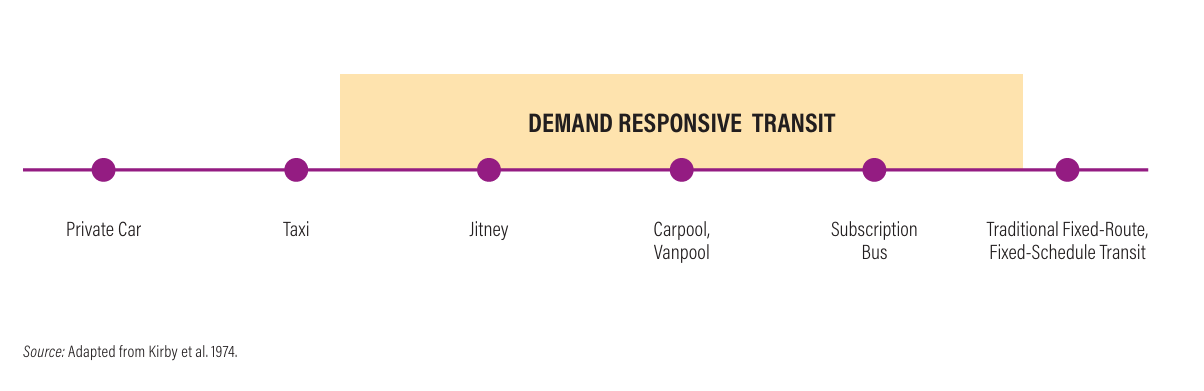
\includegraphics[width=0.9\textwidth]{fig_drt_spectrum.png}
\caption{DRT positioned within the transport-mode spectrum (adapted from Kirby et al., 1974)}
\label{fig:drt-spectrum}
\end{figure}

\subsubsection{DRT Attributes}

DRT attributes are the flexible, tech-enabled features distinguishing it from
fixed-route service: route flexibility, request method, geographical coverage,
payment methods, vehicle type, pricing models, real-time operations, booking and
reservation method, capacity and efficiency, integration with other transport
modes, environmental impact, and level of automation. Route flexibility allows
vehicles to adjust paths in real time based on pick-up/drop-off requests, typically
booked via mobile apps; pricing is dynamic (distance-, time-, and demand-based);
vehicles range from vans and minibuses to electric and autonomous vehicles; and some
systems are progressing toward driverless automation to reduce cost and improve
operational precision.

\subsubsection{Global View of DRT}

An initial global survey identified 151 operational DRT cases worldwide. Europe
accounts for the largest regional share, while the United States and Australia lead
at the country level in systems targeting specific demand segments
(Figure~\ref{fig:regional-dist}). Of the 151 systems, 92 serve the general public,
26 serve targeted demand segments (elderly, disabled, students), and 33 are hybrid.
DRT adoption remains concentrated in developed countries, with limited presence in
India, Brazil, Mexico, Egypt, Bangladesh, and Indonesia, a disparity suggesting
significant untapped potential in lower-income regions.

\begin{figure}[H]
\centering
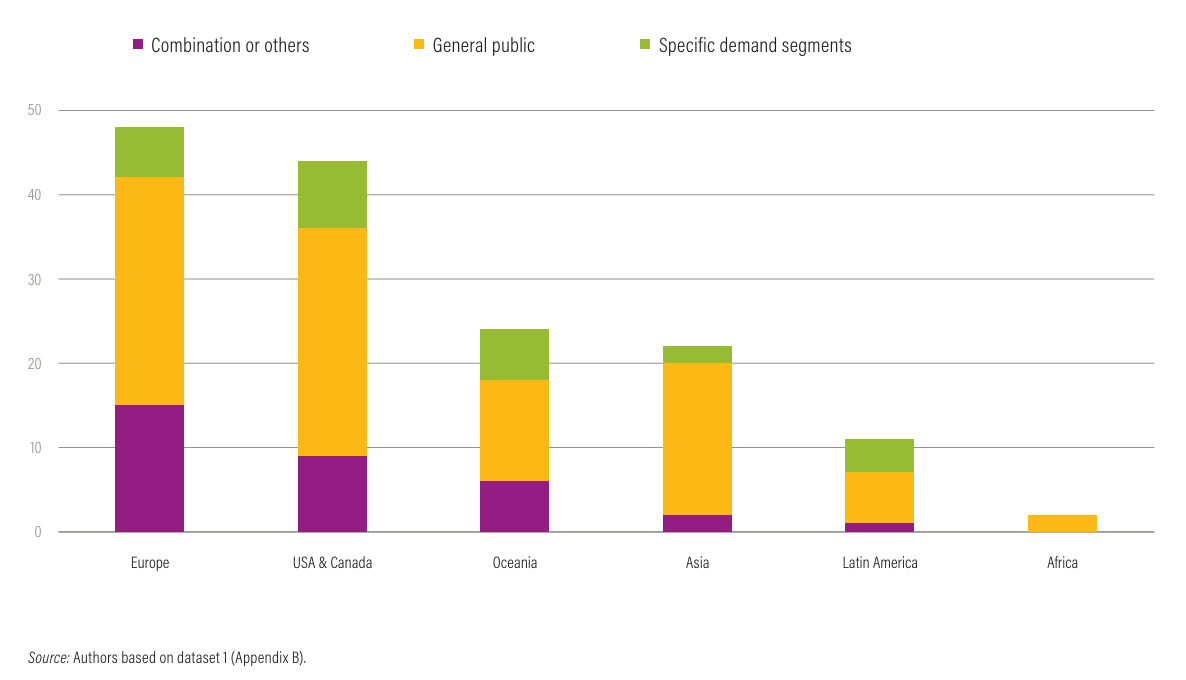
\includegraphics[width=\textwidth]{fig_regional_distribution.png}
\caption{Distribution of sampled DRT types, by region (Source: authors' dataset, Appendix B of source report)}
\label{fig:regional-dist}
\end{figure}

Within India specifically, DRT services identified in the global survey are
concentrated in Bengaluru, Chennai, Delhi-NCR, Hyderabad, Kolkata, Mumbai, and Pune,
almost all classified as ``General Public'' services (Table~\ref{tab:drt-india}).
Notably, every identified DRT operator in India is privately owned, with no
government-integrated or policy-based DRT system identified, suggesting private
companies are filling a market gap that policy has not yet addressed.

\begin{table}[H]
\centering
\small
\caption{DRT systems operating in India (Source: authors' dataset, Appendix B of source report)}
\label{tab:drt-india}
\begin{tabular}{@{}cp{1.5cm}p{1.8cm}p{1.9cm}p{3.7cm}p{2.8cm}@{}}
\toprule
\textbf{\#} & \textbf{Region} & \textbf{Country} & \textbf{City} & \textbf{System name} & \textbf{Type of service} \\
\midrule
1  & Africa & Egypt & Cairo & Careem Bus & General Public \\
2  & Africa & Egypt & Cairo & UberBus & General Public \\
3  & Asia & Bangladesh & Dhaka & Pipeep & General Public \\
4  & Asia & India & Bengaluru & ZipGo & General Public \\
5  & Asia & India & Chennai & Shuttl & General Public \\
6  & Asia & India & Delhi-NCR & Shuttl & General Public \\
7  & Asia & India & Hyderabad & Easy Commute & General Public \\
8  & Asia & India & Hyderabad & Shuttl & General Public \\
9  & Asia & India & Kolkata & Shuttl & General Public \\
10 & Asia & India & Mumbai & CityFlo & Combination or others \\
11 & Asia & India & Mumbai & Kruze & General Public \\
12 & Asia & India & Mumbai & Mahindra \& Mahindra (Glyd) & General Public \\
13 & Asia & India & Mumbai & Shuttl & General Public \\
14 & Asia & India & Pune & Office Ride & Specific demand segments \\
15 & Asia & India & Pune & Shuttl & General Public \\
\bottomrule
\end{tabular}
\end{table}

\subsubsection{Institutional Framework}

Successful DRT implementation depends on the institutional dimension: how the
system is organised, regulated, and related to other transport systems. Mulley et
al.\ (2012) distinguish \textbf{top-down approaches}, in which government plays the
key role in planning and defining services as public policy, from
\textbf{bottom-up approaches}, in which private operators introduce flexible
services in response to market needs. Table~\ref{tab:private-vs-public} compares
these two institutional models, and Figure~\ref{fig:institutional-quadrant} maps
three resulting operational models, namely Competitor, Supplementary, and Substitute,
against the axes of market/policy origin and integration with public transport.

\begin{table}[H]
\centering
\caption{Private Company Services versus Public Policy-Based Systems}
\label{tab:private-vs-public}
\small
\begin{tabular}{p{2.8cm}p{5.8cm}p{5.8cm}}
\toprule
 & \textbf{Private Company Services} & \textbf{Public Policy-Based Systems} \\
\midrule
Purpose & Serve market segments not covered by regular public transit & Planned as part of existing public transport, often as feeder services \\
Main characteristic & Compete with ride-hailing (Uber) and traditional public transit & Supplement or replace existing transport using advanced technology \\
Fare system & Usually do not integrate fares with other public transit & Typically integrate fares with existing public transit or offer at no charge \\
Location & More common in developing countries & More common in developed countries \\
Examples & Shuttl, CityFlo, Jetty, Uber Bus (India, Mexico, Brazil, Egypt) & TAD IDMF, FlexHop, R\'eSaTao, Bridj, Keoride (France, Australia, USA) \\
\bottomrule
\end{tabular}
\end{table}

\begin{figure}[H]
\centering
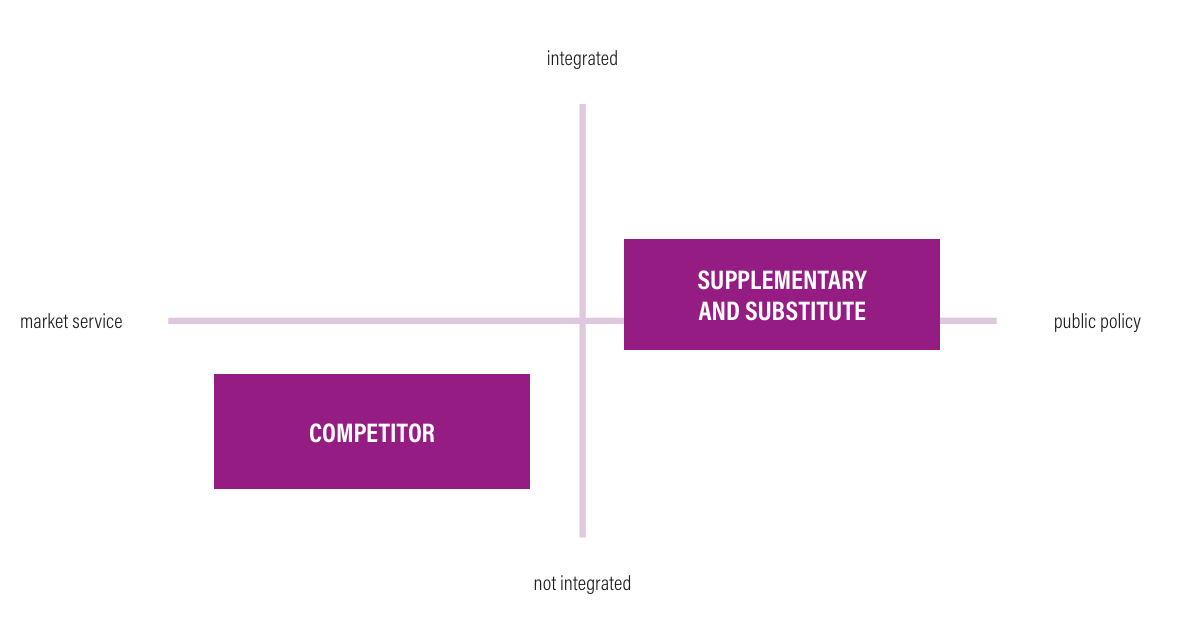
\includegraphics[width=0.85\textwidth]{fig_institutional_quadrant.png}
\caption{DRT models: institutional origin and integration with public transport}
\label{fig:institutional-quadrant}
\end{figure}

CityFlo in Mumbai exemplifies a blend of the Competitor and Supplementary models: it
competes with regular buses and ride-hailing through flexible shuttle services on
scheduled routes, while operating with a separate fare system rather than
integrating with public transit fares, following the general pattern of private
DRT initiatives in other developing countries (Shuttl, Uber Bus).

\subsection{Sustainability in DRT and the Dubai Bus-on-Demand Case Study}

DRT supports sustainable urban mobility by bridging the gap between the flexibility
of private transport and the affordability of public systems.
\textbf{Environmentally}, it reduces congestion and emissions through shared rides,
electric/autonomous vehicles, and real-time route optimisation. \textbf{Socially},
it enhances access for underserved populations, namely rural, low-income, elderly, and
disabled users, supporting equitable access to jobs, education, and healthcare.
\textbf{Economically}, sustainability depends on balancing operating costs with
fare revenue; the Cost Recovery Ratio (CRR) is a key metric for financial viability.

The \textbf{Dubai Bus-on-Demand (DBOD)} service, operating since February 2020 under
a Public-Private Partnership, offers a practical illustration of these principles.
The service uses 12--14-seat wheelchair-accessible vehicles with fares based on
service kilometres. Capacity utilisation increased by 23.5\% from 2020 to 2021,
with hourly utilisation reaching 8+ riders per vehicle per hour, among the highest
of any global micro-transit service. Figure~\ref{fig:dubai-case} summarises the key
operational results.

\begin{figure}[H]
\centering
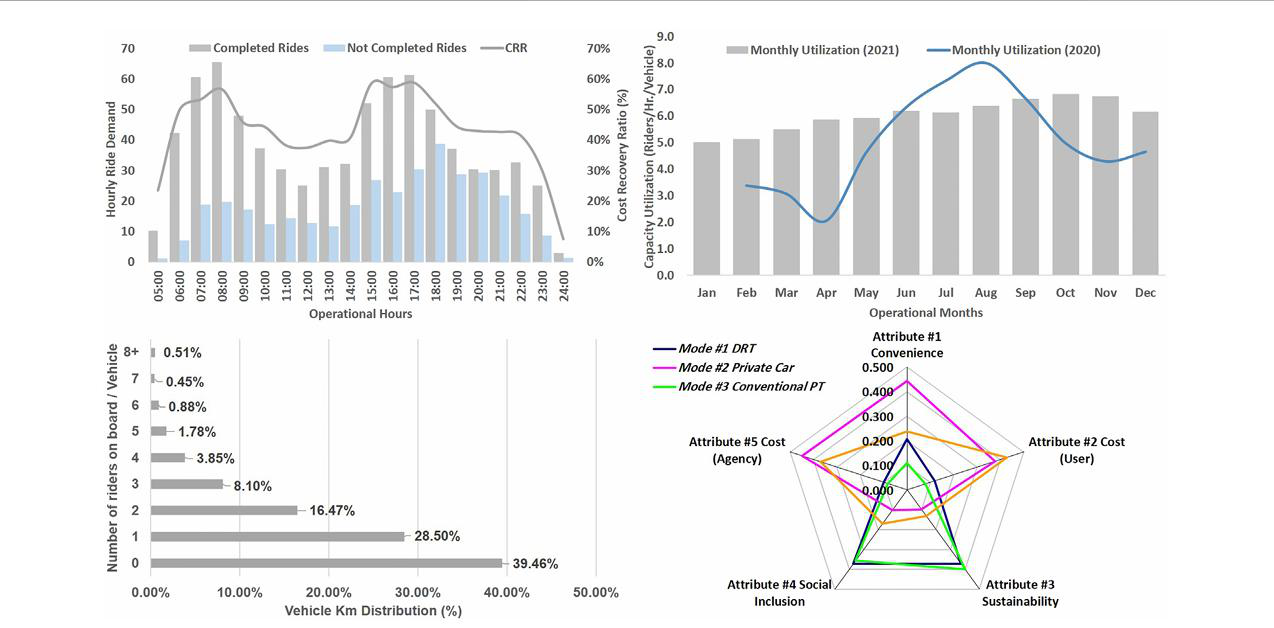
\includegraphics[width=\textwidth]{fig_dubai_case_study.png}
\caption{Results from the Dubai Bus-on-Demand case study: hourly ride demand and cost
recovery ratio, monthly capacity utilisation (2020 vs.\ 2021), vehicle-km
distribution by occupancy, and comparative mode attributes}
\label{fig:dubai-case}
\end{figure}

Three factors emerged as critical to commercial sustainability: (1) \textbf{mode
choice}, balancing sustainability and social-inclusion attributes against
user-specific needs; (2) \textbf{integrated planning for cost recovery}, where CRR is
typically higher during high-demand peak hours and struggles during off-peak
service; and (3) \textbf{service efficiency}, where smaller vehicles (e.g., Toyota
Hiaces) improved Expected Time of Arrival and vehicle utilisation relative to larger
buses, which struggled with constraints such as U-turns.

\subsection{Challenges and Limitations of DRT}

Despite its promise, DRT faces several persistent challenges: a lack of
standardised definition or categorisation (making comparative analysis difficult),
operational complexity in achieving genuinely effective real-time responsiveness,
regulatory and financial integration challenges (particularly in developing
regions), and limited comprehensive data for cross-context comparative studies.

\subsection{What is Demand in DRT?}

Demand in DRT refers to the number, timing, location, and characteristics of trip
requests made by users of flexible, on-call transit services. Unlike fixed-route
transit, where demand is largely shaped by supply (schedules and routes), DRT
demand is dynamic, decentralised, and multi-dimensional, requiring active
participation from users who define their own trip origins, destinations, and
desired timings (Alsaleh \& Farooq, 2021). Table~\ref{tab:drt-vs-frt} contrasts DRT
and fixed-route transit (FRT) across the key planning dimensions.

\begin{table}[H]
\centering
\caption{Demand in DRT versus Fixed-Route Transit (FRT)}
\label{tab:drt-vs-frt}
\small
\begin{tabular}{p{3cm}p{5.5cm}p{5.5cm}}
\toprule
\textbf{Aspect} & \textbf{DRT} & \textbf{FRT} \\
\midrule
Service model & On-demand, dynamically routed & Pre-scheduled, fixed routes/stops \\
User role & Active: users request rides via apps/calls & Passive: users adjust to fixed routes \\
Routing & Flexible, real-time adjustment & Static, rarely adjusted \\
Demand nature & Uncertain, fluctuates in time/space & Predictable, based on historical patterns \\
System responsiveness & High: responds instantly & Low: delayed by timetable revisions \\
Service coverage & Can target low-density/underserved areas & Economical only in high-density corridors \\
Infrastructure need & Light: efficient dispatch, digital booking & Heavy: fixed stops, signage, schedules \\
Cost efficiency & Efficient when demand is clustered & More cost-efficient in high-demand peaks \\
Technology use & High: GPS, apps, real-time algorithms & Moderate: mostly scheduling/fare collection \\
Performance metrics & Wait time, detour length, ride acceptance & Schedule adherence, ridership per trip \\
\bottomrule
\end{tabular}
\end{table}

\subsubsection{Key Aspects of Demand in DRT Systems}

\begin{enumerate}[nosep]
  \item \textbf{Temporal aspects:} demand peaks during morning/evening commutes,
    with weekday/weekend and seasonal variation requiring dynamic scheduling.
  \item \textbf{Spatial aspects:} residential zones generate early-morning
    requests; commercial/institutional areas are high-demand destinations during
    the day, producing one-way patterns and vehicle repositioning needs.
  \item \textbf{User demographics and socioeconomic characteristics:} older
    adults, low-income populations, and car-less households rely more heavily on
    DRT.
  \item \textbf{Trip purpose:} regular commuters show predictable patterns;
    health, leisure, or shopping trips are more spontaneous and dispersed.
  \item \textbf{Event-driven and external factors:} concerts, sports matches,
    weather, or transit strikes trigger sudden demand spikes requiring real-time
    fleet adjustment.
  \item \textbf{Mode-shift behaviour:} DRT attracts users from other modes when
    fixed-route transit is inadequate, serving as both a primary mode and a
    complementary connector.
\end{enumerate}

\subsubsection{Assessing Demand Viability}

Because a ride request does not automatically signal meaningful or sustainable
demand, operators must assess indicators such as repeat usage, duration of demand,
trip-purpose diversity, and unmet (latent) demand (Table~\ref{tab:viability}).

\begin{table}[H]
\centering
\caption{Indicators for Judging Demand Viability in DRT}
\label{tab:viability}
\small
\begin{tabular}{p{4.5cm}p{9cm}}
\toprule
\textbf{Indicator} & \textbf{What It Reveals} \\
\midrule
Repeat users & Ongoing utility and user satisfaction \\
Duration of demand & Temporal stability (beyond trial or event-driven usage) \\
Trip purpose diversity & Coverage of essential needs (work, health, school) \\
Daily/weekly consistency & Demand regularity across different days and hours \\
Unmet demand (latent users) & Potential growth if supply or awareness is improved \\
\bottomrule
\end{tabular}
\end{table}

Low ridership does not necessarily reflect low demand. In the Indian context,
suburban connectivity gaps (e.g., Mankhurd--Panvel corridor, where last-mile access
to suburban rail is weak and costly), unreliable public bus systems in cities like
Patna and Bhopal (where informal e-rickshaws are often cheaper for short trips), and
suppressed women's ridership in rural India (due to safety concerns and poor
lighting) all illustrate how ridership figures can significantly understate true
transit demand.

\subsection{Demand--Supply Equilibrium in DRT}

Demand--supply equilibrium is a dynamic state where a DRT system's transport
capacity, namely vehicles, drivers, and routing coverage, aligns with passengers'
travel needs in time, location, and frequency. If supply exceeds demand, idle
fleets and unnecessary operating costs result; if demand exceeds supply, wait times
lengthen, trips are missed, and satisfaction drops. Table~\ref{tab:supply-align}
shows how specific demand signals should guide supply responses, and
Table~\ref{tab:supply-components} summarises the key supply-side components that
must be balanced.

\begin{table}[H]
\centering
\caption{Aligning Supply with DRT Demand Signals}
\label{tab:supply-align}
\small
\begin{tabular}{p{6cm}p{7.5cm}}
\toprule
\textbf{Observed Demand Pattern} & \textbf{Suggested Supply Response} \\
\midrule
High elderly population usage & Small vehicles, shorter detours, door-to-door service \\
Dense, short-trip clusters & Frequent ride pooling, high vehicle turnover \\
Time-bound work commutes & Scheduled fleet bursts during peak hours \\
Uneven area demand distribution & Dynamic vehicle repositioning \\
Night-time safety concerns & Incentivised night shifts or guaranteed availability \\
\bottomrule
\end{tabular}
\end{table}

\begin{table}[H]
\centering
\caption{Key Supply Components in DRT: Role in Balancing Supply}
\label{tab:supply-components}
\small
\begin{tabular}{p{3.5cm}p{10cm}}
\toprule
\textbf{Aspect} & \textbf{Role in Balancing Supply} \\
\midrule
Fleet size \& type & Vehicles (vans, e-rickshaws) matched to demand without overloading during low-use periods \\
Operating hours & Flexible shifts for early commutes or late-night travel \\
Dispatching system & GPS-based trip matching and real-time control-centre coordination \\
Routing algorithms & Smart clustering and re-routing to optimise shared rides, reduce idle time \\
Fare \& incentives & Pricing strategies (discounts, surge pricing) to regulate demand and encourage usage \\
\bottomrule
\end{tabular}
\end{table}

Achieving this balance relies on mathematical demand-supply models, agent-based
simulations of passenger/operator behaviour, and machine-learning techniques that
forecast short-term surges from web activity, weather, or local events.

\subsection{Evolution of Demand Modelling in DRT Systems: A Four-Phase Analysis}

Demand prediction is fundamental to efficient DRT operation: without regional
demand predictions, the gap between passengers' desired and actual boarding times
widens significantly, producing inefficient service with minimal movement and
maximum cost. The evolution of demand-modelling approaches can be traced through
four phases.

\subsubsection{Phase 1: Early Static Prediction Models (Pre-2010s)}
The earliest models relied on rule-based algorithms with static assumptions. The
Dial-a-Ride Problem (DARP) framework emerged as the fundamental approach for
optimising routes under fixed constraints (vehicle capacity, time windows). These
models suffered from static demand assumptions, inability to adapt to
spatiotemporal variation, limited consideration of passenger-specific needs, and a
lack of real-time responsiveness, especially problematic in suburban areas where
demand is inherently sparse and heterogeneous.

\subsubsection{Phase 2: Statistical Forecasting Era (2010--2018)}
This phase saw the application of time-series analysis (ARIMA/ETS models),
multi-variable regression, and demand-classification metrics (ADI/CV\textsuperscript{2}).
These methods improved temporal forecasting but still struggled with spatial
dependencies and heterogeneous demand. As Makridakis et al.\ observed, statistical
methods like ARIMA showed ``superiority for stationary urban demand'' but ``failed
for erratic rural demand'', precisely where DRT services are often most needed.

\subsubsection{Phase 3: Heuristic and Optimization Models (2018--2022)}
The third phase introduced sophisticated multi-objective optimisation approaches.
The Search and Rescue Algorithm (SaRA), a heuristic technique inspired by human
search-and-rescue behaviour, divides the search space into sub-spaces and assigns
``search and rescue workers'' to explore them, enabling problem spaces to be
effectively divided and conquered and non-promising regions to be efficiently
eliminated. Zigrand et al.\ combined demand clustering with a dynamic DaRP solver,
improving insertion rates by 3.5\% in suburban areas, demonstrating that
geographical/temporal clustering can mitigate data sparsity and that look-ahead
optimisation outperforms traditional myopic insertion heuristics.

\subsubsection{Phase 4: Machine Learning Revolution (2022--Present)}
The most recent phase has seen remarkable advances in machine learning tailored
explicitly for DRT demand prediction. The PGDRT model (Prediction Demand based on
Graph Convolutional Network) uses both spatial characteristics (proximity between
regions, transportation convenience, functional similarity between areas) and
temporal characteristics (adjacent visual characteristics, periodic patterns,
representative past-demand features). Because DRT data are inherently sparse due to
spatiotemporal effects, Lee et al.\ employed channel-wise attention and temporal
means to alleviate data sparsity before applying ConvLSTM. Other innovations include
Deep-DRT (neural networks for multidimensional data), hybrid VAR-CNN models for
suburban areas, and spatiotemporal Graph Convolutional Networks that reduced
boarding-time gaps by 18\%, with some approaches achieving 95\% R\textsuperscript{2}
accuracy despite sparse data.

\subsubsection{Critical Challenges and Future Directions}
Four challenges recur across the literature: (1) \textbf{data sparsity}, where suburban
DRT still relies on synthetic data generation to overcome extreme sparsity;
(2) \textbf{spatiotemporal dependency}, since spatial characteristics affect temporal
trends, requiring joint modelling; (3) \textbf{equity considerations}, where recent
innovations (e.g., DEMO-GRAPH) integrate demographics into demand classification to
better serve mobility-restricted passengers; and (4) \textbf{autonomous
integration}, namely DRT's potential integration with autonomous vehicles, with
projections suggesting up to 40\% cost reduction by 2030 via AI-driven fleets.

\subsection{Summary of Reviewed Literature}

Table~\ref{tab:lit-summary} summarises the fourteen distinct studies reviewed for
this seminar, spanning ride-hailing demand prediction, e-bike/DRT integration,
sustainable DRT design, transit-oriented autonomous vehicles, and suburban DRT
optimisation frameworks.

\small
\begin{longtable}{p{0.4cm}p{4.8cm}p{0.6cm}p{2.7cm}p{4.7cm}}
\caption{Summary of Reviewed Literature on DRT Demand Modelling}
\label{tab:lit-summary} \\
\toprule
\textbf{\#} & \textbf{Title / Authors} & \textbf{Yr} & \textbf{Study Area} & \textbf{Key Finding} \\
\midrule
\endfirsthead
\toprule
\textbf{\#} & \textbf{Title / Authors} & \textbf{Yr} & \textbf{Study Area} & \textbf{Key Finding} \\
\midrule
\endhead
\bottomrule
\endfoot
1 & Demand Prediction of Ride-Hailing Pick-Up Location Using Ensemble Learning; Carson-Bell et al. & 2021 & Chicago, USA & Ensemble/neural models predict demand accurately under privacy constraints; reduced dead-mileage and idle time \\
2 & Combination of e-bike-sharing and DRT in rural areas; Bruzzone et al. & 2021 & Velenje, Slovenia & Integrated DRT + e-bike-share increased mobility access and was perceived positively by users \\
3 & The journey of demand-responsive transportation: towards sustainable services; Deka et al. & 2023 & Dubai, UAE & Cost Recovery Ratio is the most critical sustainability indicator; smaller vehicles increase ETA efficiency \\
4 & DRT for Urban Mobility: Integrating Mobile Data Analytics; Melo, Gomes, Abbasi, Arantes & 2024 & Porto, Portugal & Data-driven framework reduced stops by 135\%, distance by 81\%, wait times by 163\%, carbon footprint by 73\% \\
5 & Real-Time Taxi Demand Prediction Using Data from the Web; Markou, Rodrigues, Pereira & 2018 & New York City, USA & Fusing event data with time-series models improved prediction (MAE reduced $\sim$37.5\%) \\
6 & Transit-oriented autonomous vehicle operation with integrated demand-supply interaction; Wen et al. & 2018 & Suburban European city & Transit-oriented AV integration enhances availability, supports shared rides, reduces required fleet size by 50\% \\
7 & Real-time transit demand prediction capturing station interactions; Noursalehi, Koutsopoulos, Zhao & 2018 & London Underground (32 stations) & Dynamic factor/ensemble models captured station correlations and event impacts effectively \\
8 & Cloud-Based DRT System Using Forecasting Model; Khair, Dennai, Elmir & 2024 & (Open taxi data, Kaggle) & Pre-allocation based on predicted demand improved VM utilisation by 25\% and cut operating costs \\
9 & Improving demand-responsive transit services: insights from the London field test; Zahedi, Koutsopoulos, Ma & 2024 & GoSutton DRT pilot, London & Joint DRT-paratransit consolidation cut fleet by 8\% and VKT by 13\% \\
10 & DRT Services for Improving Public Transport in Suburban Areas; Capodici, Migliore, D'Angelo, D'Orso & 2022 & Palermo, Italy & DRT-rail integration improves modal share, especially for non-drivers and women; 28.2\% more job access \\
11 & Demand Forecasting for Suburban DRT Services; Univ.\ of Palermo Transport Systems Lab & 2022 & Palermo, Italy & Spatiotemporal clustering identified efficient zone-formation strategies and fleet performance \\
12 & Optimization-driven Demand Prediction Framework for Suburban DRT Systems; Zigrand et al. & 2023 & Suburbs of large French cities & Forecast-informed, optimisation-embedded ML gave 3.5\% improvement in insertion rate \\
13 & A Multi-task Deep Learning Framework for Sparse DRT Demand; Lee, Choi, Kim & 2024 & Yeongjongdo, Incheon, Korea & Zero-inflated, multi-task deep learning improved prediction by focusing on sparse OD-pair demand \\
14 & Short-Term Prediction of Demand for Ride-Hailing Services (UberNet); Chen, Thakuriah, Ampoutolas & 2021 & New York City (Uber data) & CNN-based UberNet outperformed traditional and neural models using embedded spatiotemporal features \\
\end{longtable}
\normalsize

\section{Case Study: On-Demand Transit in Belleville, Ontario}

\subsection{Background of the Study}

\textbf{Title of Paper:} Interpretable data-driven demand modelling for on-demand
transit services\\
\textbf{Authors:} Nael Alsaleh, Bilal Farooq\\
\textbf{Journal:} Transportation Research Part A (Policy and Practice), Volume 154,
Pages 1--22 (2021)

The Greater Toronto and Hamilton Area (GTHA), home to more than 6.9 million people,
is one of Canada's largest and most populous regions. Approximately 43\% of its
population resides in dense urban areas, while the remaining 57\% live in
low-density regions that make up 96\% of the total land area, a pattern common to
many countries, including India. In these low-density areas, traditional
fixed-route public transit (FRT) struggles to operate efficiently: low frequency and
limited coverage make service inconvenient, particularly during off-peak hours and
in suburban or rural zones.

\subsubsection{Research Problem Statement}
Traditional fixed-route buses or trains cannot efficiently serve low-demand areas
due to high operational costs and vehicle underutilisation during off-peak times,
an issue especially acute for shift workers who need transport when conventional
transit is scarce. On-demand transit (ODT) has emerged as a cost-effective,
flexible, demand-responsive alternative, already implemented in several Canadian
cities including Regina, Saskatoon, Calgary, and Chatham-Kent. While these services
show promise, there remains a lack of in-depth research on demand modelling for
dedicated-fleet ODT services specifically, the gap this study addresses.

\subsubsection{Objectives and Scope}
The study develops robust trip-production and trip-distribution models for ODT
services, focused on predicting daily trip volumes and understanding how trips are
distributed across geographic areas. It investigates how demographic factors
(population density, income, working-age population share) and trip characteristics
(distance, purpose, time of day) influence demand, using Random Forest, Artificial
Neural Networks (ANN), and Deep Neural Networks (DNN), with SHAP analysis used to
interpret variable contributions, addressing a gap in interpretable demand
modelling tailored specifically to dedicated ODT services.

\subsection{Study Area: City of Belleville, Ontario}

Belleville is located in Eastern Ontario, about 190 km east of Toronto, and is the
largest urban centre in the Quinte region (Figure~\ref{fig:belleville-map}). The
city spans 246.8 sq.\ km with a population density of 205.1 people per sq.\ km. As
per the 2016 Census, Belleville has a population of 50{,}716, with 63\% in the
working-age group (15--64 years); median after-tax household income is CAD
53{,}367, below the Canadian national average of CAD 61{,}348.

\begin{figure}[H]
\centering
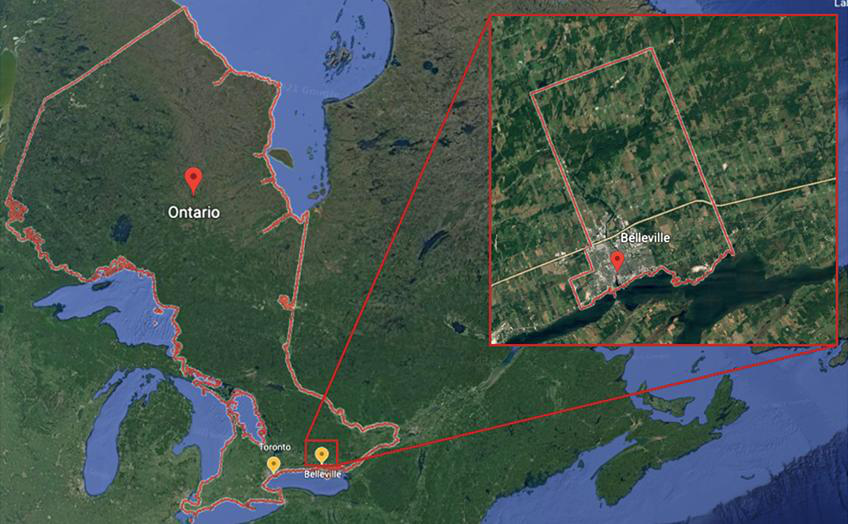
\includegraphics[width=0.7\textwidth]{fig_belleville_map.png}
\caption{City of Belleville, Ontario, within the Greater Toronto and Hamilton Area}
\label{fig:belleville-map}
\end{figure}

Belleville's transit system includes 10 fixed routes operated by a fleet of 16
buses. In January 2018, Route 11 was launched as a late-night fixed-route service
(9:30 PM--12:30 AM) using two 40-ft buses running every 30 minutes; in September
2018, this service was converted into an ODT pilot to reduce costs and improve
efficiency (Pantonium, 2019; Sanaullah et al., 2021). The ODT service retains the
same 40-ft buses, stops, and fare (CAD 3) as the previous fixed-route system, but
operates on demand from 9:00 PM to 12:00 AM on weekdays and 7:00 PM to 12:00 AM on
weekends, with routing dynamically adjusted based on real-time passenger requests
booked through an app, phone, or at-stop boarding. Figure~\ref{fig:belleville-services}
contrasts the fixed and on-demand service footprints.

\begin{figure}[H]
\centering
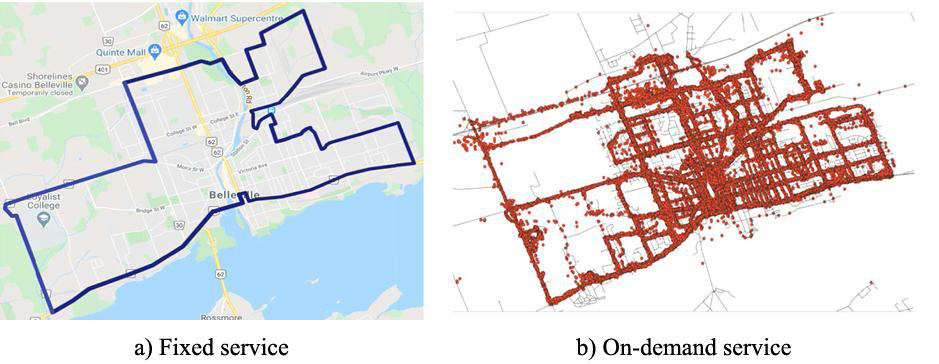
\includegraphics[width=\textwidth]{fig_belleville_services.png}
\caption{Belleville public transit: (a) fixed-route service coverage; (b) on-demand
service pickup/drop-off point density}
\label{fig:belleville-services}
\end{figure}

The transition to ODT resulted in a sustained increase in demand, driven by
enhanced flexibility in routing and broader service coverage.

\subsection{Methodology and Model Specifications}

\subsubsection{Data Preparation}
The study uses operational data from Belleville's ODT system collected between
18 September 2018 and 29 May 2019, combined with demographic data from the 2016
Census. The dependent variables are trip production (daily trips generated per
dissemination area, DA) and trip distribution (daily trips between area pairs).
Explanatory variables span demographic characteristics for both trip origin and
destination (population density, median income, average household size, percentage
of males, working-age percentage) and trip characteristics (hours of operation per
day, day of week, month of year). Table~\ref{tab:descriptive-stats} summarises the
descriptive statistics for all variables.

\begin{table}[H]
\centering
\caption{Descriptive Statistics for Explanatory and Dependent Variables}
\label{tab:descriptive-stats}
\small
\begin{tabular}{p{5.3cm}p{2.6cm}p{1cm}p{1cm}p{1.8cm}p{1.5cm}}
\toprule
\textbf{Variable} & \textbf{Unit} & \textbf{Min} & \textbf{Max} & \textbf{Mean} & \textbf{Std.\ Dev.} \\
\midrule
\multicolumn{6}{l}{\textit{Dependent Variables}} \\
Trips produced per DA per day & count & 1 & 35 & 4.3 & 5.29 \\
Trips between any two DAs per day & count & 1 & 11 & 2.4 & 1.18 \\
\multicolumn{6}{l}{\textit{Demographic Characteristics (Origin)}} \\
Population density & people/km\textsuperscript{2} & 63.2 & 8{,}139.8 & 1{,}700.7 & 1{,}628.02 \\
Median income & CAD & 24{,}640 & 87{,}296 & 49{,}506.2 & 13{,}522.32 \\
Average household size & count & 1.5 & 2.8 & 2.2 & 0.30 \\
Percentage of males & \% & 37.2 & 56.8 & 47.2 & 4.24 \\
Working-age percentage & \% & 38.9 & 80.7 & 63.5 & 8.52 \\
\multicolumn{6}{l}{\textit{Demographic Characteristics (Destination)}} \\
Population density & people/km\textsuperscript{2} & 63.2 & 8{,}139.8 & 2{,}075 & 2{,}094.04 \\
Median income & CAD & 24{,}640 & 87{,}296 & 46{,}851.6 & 13{,}407.37 \\
Average household size & count & 1.5 & 2.8 & 2.17 & 0.25 \\
Percentage of males & \% & 37.2 & 56.8 & 47.5 & 3.93 \\
Working-age percentage & \% & 38.9 & 80.7 & 66.4 & 6.54 \\
\multicolumn{6}{l}{\textit{Trip Characteristics}} \\
Hours of operation per day & binary (0/1) & 0 & 1 & -- & -- \\
Day of the week & discrete (1--7) & 1 & 7 & -- & -- \\
Month of the year & discrete (1--9) & 1 & 9 & -- & -- \\
\bottomrule
\end{tabular}
\end{table}

\subsubsection{Model Development}
Four machine-learning algorithms, namely Random Forest (RF), Bagging, Artificial Neural
Network (ANN), and Deep Neural Network (DNN), were used to model daily trip
production and distribution. RF and Bagging are ensemble methods that construct
multiple decision trees and combine their outputs; RF selects a random feature
subset at each node split, while Bagging uses all available features (Gislason et
al., 2006).

\subsubsection{Demand Clustering}
K-means clustering classified trip production and distribution into three demand
clusters based on frequency, namely Low (1 trip/day), Medium (2--5 trips/day), and High
(more than 5 trips/day), with the optimal cluster count ($K=3$) confirmed via the
Elbow Method. For trip production, the low-demand cluster was most common (40\% of
daily trips), followed by medium (36\%) and high (24\%). For trip distribution,
high-level distribution (more than two trips/day between areas) accounted for 39\%,
medium for 37\%, and low for 24\%. Figures~\ref{fig:trip-production-clusters} and
\ref{fig:trip-distribution-clusters} show the clustering analysis for production and
distribution respectively.

\begin{figure}[H]
\centering
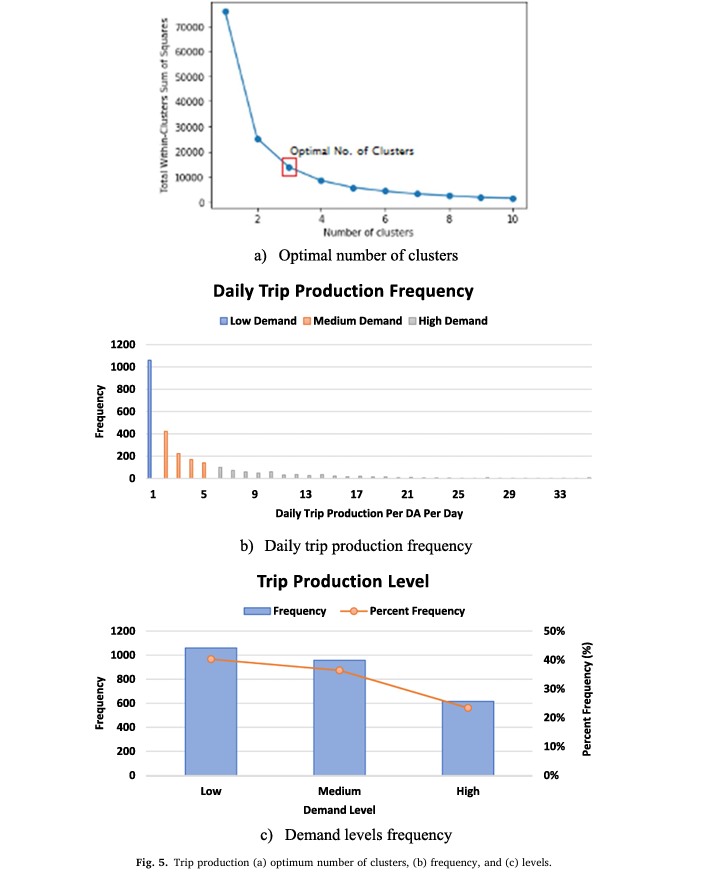
\includegraphics[width=0.7\textwidth]{fig_trip_production_clusters.png}
\caption{Trip production: (a) optimum number of clusters, (b) daily frequency
distribution, (c) demand-level frequency}
\label{fig:trip-production-clusters}
\end{figure}

\begin{figure}[H]
\centering
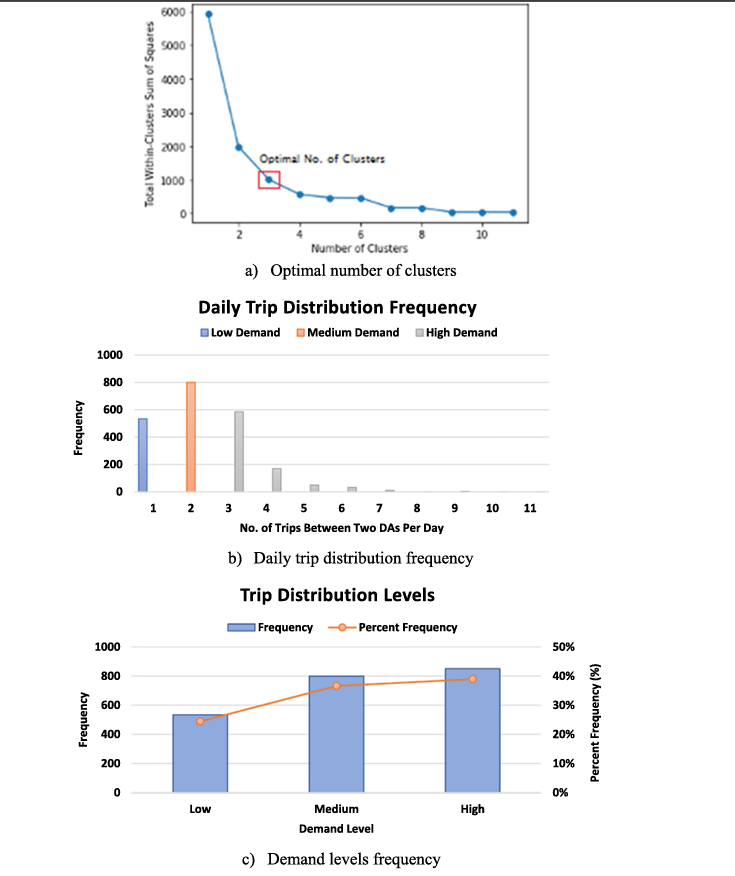
\includegraphics[width=0.7\textwidth]{fig_trip_distribution_clusters.png}
\caption{Trip distribution: (a) optimum number of clusters, (b) daily frequency
distribution, (c) demand-level frequency}
\label{fig:trip-distribution-clusters}
\end{figure}

Key takeaways from the clustered data were that demand shows strong temporal
variation by time of day and day of week (particularly for high-demand levels),
that demographic factors such as population density and income levels significantly
influenced demand patterns, and that optimal fleet deployment during peak hours was
essential to maintaining service efficiency.

\subsubsection{Hyperparameter Tuning and Model Evaluation}
Hyperparameters for the four algorithms were tuned using Bayesian Optimization,
which reduces the number of evaluations required by intelligently exploring the
search space, compared to manual tuning or exhaustive Grid/Random Search (Snoek et
al., 2012; Yang \& Shami, 2020). Figure~\ref{fig:hyperparameters} lists the
hyperparameter sets explored for each algorithm. The dataset was split into
training and testing subsets in a 4:1 ratio, with 10-fold cross-validation used
during model evaluation to ensure robustness and prevent overfitting.

\begin{figure}[H]
\centering
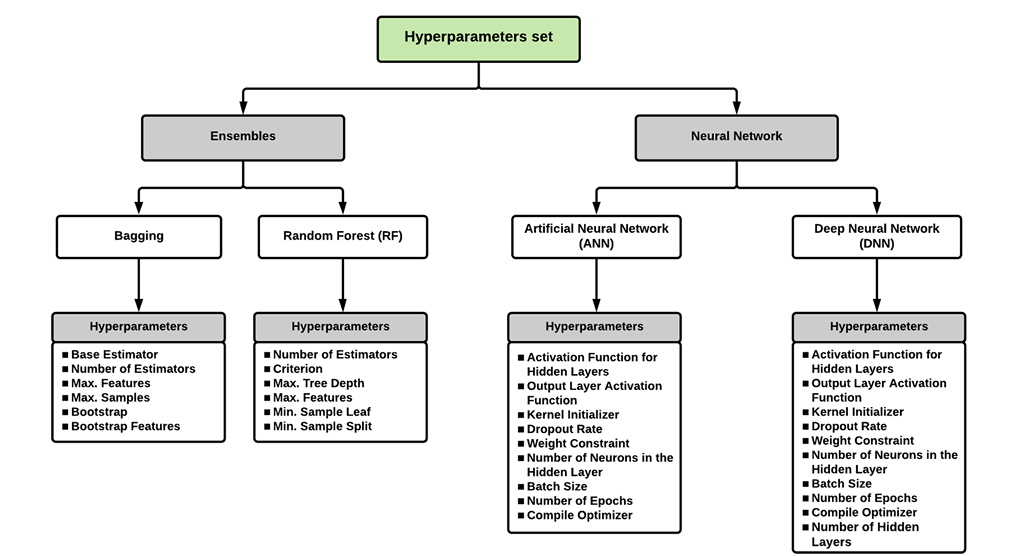
\includegraphics[width=0.85\textwidth]{fig_hyperparameters.png}
\caption{Hyperparameter sets explored for RF, Bagging, ANN, and DNN}
\label{fig:hyperparameters}
\end{figure}

Model interpretability was assessed using SHAP (SHapley Additive exPlanations),
which explains model outputs by calculating the average marginal contribution of
each explanatory variable to the predictions (Lundberg \& Lee, 2017).

\subsection{Results of the ODT Daily Trip Production and Distribution Models}

Figure~\ref{fig:model-comparison} compares the predictive accuracy of RF, Bagging,
ANN, and DNN across the low, medium, and high demand levels for the trip
production model; all four algorithms show a consistent dip in accuracy for the
medium-demand level, reflecting boundary misclassification between adjacent demand
classes.

\begin{figure}[H]
\centering
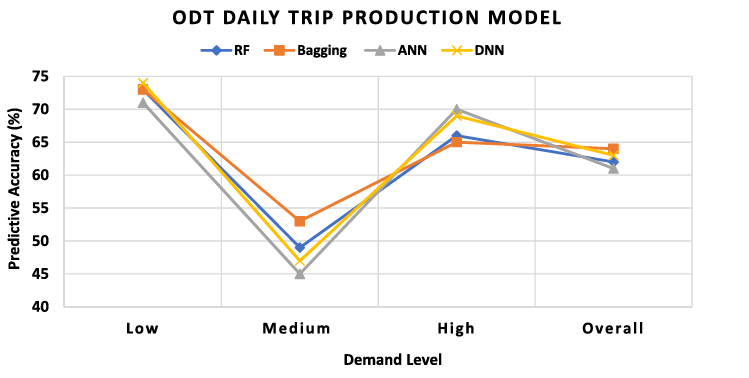
\includegraphics[width=0.75\textwidth]{fig_model_comparison.png}
\caption{Comparing the predictive accuracy of the ODT daily trip production models}
\label{fig:model-comparison}
\end{figure}

Table~\ref{tab:production-perf} summarises algorithm-wise performance for the trip
production model, and Table~\ref{tab:production-confusion} gives the detailed
confusion matrix for the best-performing algorithm (Bagging).

\begin{table}[H]
\centering
\caption{Trip Production Model: Algorithm Performance Comparison}
\label{tab:production-perf}
\small
\begin{tabular}{p{1.9cm}p{1.5cm}p{1.7cm}p{1.5cm}p{1.5cm}p{4.8cm}}
\toprule
\textbf{Algorithm} & \textbf{Acc.\ Low} & \textbf{Acc.\ Medium} & \textbf{Acc.\ High} & \textbf{Overall} & \textbf{Challenges} \\
\midrule
DNN & 74\% & 45\% & 60\% & 64\% & Medium-level misclassification (2 trips/day boundary) \\
Bagging & 68\% & 53\% & 61\% & 64\% & Lower accuracy for medium production level \\
ANN & 72\% & 50\% & 70\% & 62\% & -- \\
Random Forest & 70\% & 51\% & 65\% & 63\% & -- \\
\bottomrule
\end{tabular}
\end{table}

\begin{table}[H]
\centering
\caption{Trip Production Model Testing Confusion Matrix (Bagging Algorithm)}
\label{tab:production-confusion}
\small
\begin{tabular}{p{3cm}p{2cm}p{2.2cm}p{2cm}p{1.5cm}p{1.8cm}}
\toprule
\textbf{Predicted} $\rightarrow$ & \textbf{Low} & \textbf{Medium} & \textbf{High} & \textbf{Total} & \textbf{Acc.\ (\%)} \\
\midrule
Low Demand & 107 & 3 & 3 & 113 & 64 \\
Medium Demand & 32 & 109 & 27 & 168 & 65 \\
High Demand & 14 & 44 & 98 & 156 & 70 \\
Total & 153 & 156 & 128 & 437 & 64 \\
\bottomrule
\end{tabular}
\end{table}

For trip distribution, Table~\ref{tab:distribution-perf} shows RF was the best
overall performer (72\% accuracy), while DNN achieved perfect accuracy (100\%) at
the low-demand level.

\begin{table}[H]
\centering
\caption{Trip Distribution Model: Algorithm Performance Comparison}
\label{tab:distribution-perf}
\small
\begin{tabular}{p{2.3cm}p{2.4cm}p{2.4cm}p{2.4cm}p{2cm}}
\toprule
\textbf{Algorithm} & \textbf{Acc.\ Low} & \textbf{Acc.\ Medium} & \textbf{Acc.\ High} & \textbf{Overall} \\
\midrule
DNN & 100\% & 61\% & 60\% & 71\% \\
Random Forest & 70\% & 65\% & 63\% & 72\% \\
Bagging & 64\% & 59\% & 61\% & 69\% \\
ANN & 68\% & 60\% & 62\% & 69\% \\
\bottomrule
\end{tabular}
\end{table}

\begin{table}[H]
\centering
\caption{Trip Distribution Model Testing Confusion Matrix (Random Forest Algorithm)}
\label{tab:distribution-confusion}
\small
\begin{tabular}{p{3cm}p{2cm}p{2.2cm}p{2cm}p{1.5cm}p{1.8cm}}
\toprule
\textbf{Predicted} $\rightarrow$ & \textbf{Low} & \textbf{Medium} & \textbf{High} & \textbf{Total} & \textbf{Acc.\ (\%)} \\
\midrule
Low Demand & 107 & 3 & 3 & 113 & 95 \\
Medium Demand & 32 & 109 & 27 & 168 & 65 \\
High Demand & 14 & 44 & 98 & 156 & 63 \\
Total & 153 & 156 & 128 & 437 & 72 \\
\bottomrule
\end{tabular}
\end{table}

SHAP analysis (Figure~\ref{fig:shap}) identified population density as the single
most influential explanatory variable for both models, followed by percentage of
males, median income, and working-age percentage; day-of-week and month-of-year
were the least influential (Table~\ref{tab:shap-importance}).

\begin{figure}[H]
\centering
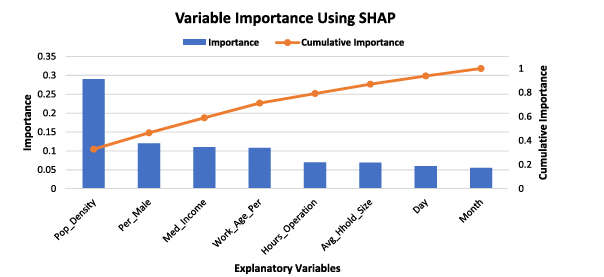
\includegraphics[width=0.75\textwidth]{fig_shap_importance.png}
\caption{Variable importance using SHAP for the trip production model}
\label{fig:shap}
\end{figure}

\begin{table}[H]
\centering
\caption{SHAP Analysis: Variable Importance Ranking}
\label{tab:shap-importance}
\small
\begin{tabular}{p{5.5cm}p{4cm}}
\toprule
\textbf{Explanatory Variable} & \textbf{Importance} \\
\midrule
Population density & Highest \\
Median income & High \\
Percentage of males & High \\
Average household size & Moderate \\
Working-age percentage & Moderate \\
Day-of-week & Least \\
Month-of-year & Least \\
\bottomrule
\end{tabular}
\end{table}

\textbf{Key findings:} the Bagging algorithm performed best for ODT daily trip
production (64\% overall accuracy); RF performed best for ODT daily trip
distribution (72\% overall accuracy); population density, median income, and
working-age percentage were the most influential variables for both production and
distribution; and DNN was most accurate at predicting the low-demand class in both
models (74\% for production, 100\% for distribution).

\subsection{Discussion and Inference}

The study reinforces prior findings that land-use and demographic characteristics
significantly affect demand for on-demand mobility services (Jain et al., 2017;
Ghaffar et al., 2020), with ODT demand higher in commercial/industrial land-use
areas, consistent with Sanaullah et al.\ (2021). It also reveals a behavioural
distinction between dedicated ODT fleets and crowdsourced mobility services: while
ride-sourcing services are commonly used for non-work-related activities, ODT users
in Belleville primarily use the service for home-to-work or home-to-shop trips.
Whereas traditional statistical methods (e.g., gravity models) are commonly used
for trip production and distribution modelling, this study demonstrates that
machine-learning algorithms such as Random Forest and Bagging offer greater
flexibility and accuracy (Pourebrahim et al., 2019); classification algorithms were
used in preference to regression due to the characteristically low, discrete demand
values observed for ODT services.

\section{Conclusion}

This seminar has traced Demand-Responsive Transit from its conceptual origins as a
flexible complement to fixed-route transit, through its operational, functional,
technological, economic, and institutional classification, to its current
global distribution, concentrated in developed countries and, within India,
almost exclusively delivered through unregulated private operators rather than
public policy. The evolution of demand-modelling techniques across four phases
(static rule-based methods, statistical forecasting, heuristic optimisation, and
the current machine-learning revolution) demonstrates how far DRT demand
prediction has advanced, while unresolved challenges of data sparsity,
spatiotemporal dependency, equity, and autonomous integration remain fertile
ground for future research.

The Belleville, Ontario case study demonstrates in concrete terms how
machine-learning models, namely Random Forest, Bagging, ANN, and DNN, can be used to
predict daily ODT trip production and distribution, and how SHAP analysis can make
such models interpretable for planners: population density, median income, and
working-age population share emerge as the dominant predictors of demand. Cities
like those in India, where public transport often misses out on large groups of
people, stand to benefit substantially from such interpretable, data-driven demand
models. Future work should aim to connect the demand side (where and when people
need rides) with the supply side (how many vehicles are needed and where), creating
a system that automatically adjusts to real-time travel needs and makes transport
more efficient, inclusive, and reliable for all users.

\begin{thebibliography}{99}

\bibitem{vuchic2007} Vuchic, V.\ R.\ (2007). \textit{Urban Transit Systems and Technology}. John Wiley \& Sons, Inc.
\bibitem{ambrosino2003} Ambrosino, G., Nelson, J.\ D., \& Romanazzo, M.\ (2003). \textit{Demand Responsive Transport Services: Towards the Flexible Mobility Agency}. ENEA.
\bibitem{balcombe2004a} Balcombe, R., et al.\ (2004). \textit{The Demand for Public Transport: A Practical Guide}. TRL Report.
\bibitem{balcombe2004b} Balcombe, R., Mackett, R., Paulley, N., Preston, J., Titheridge, H., Wardman, M., \& White, P.\ (2004). \textit{The Demand for Public Transport: A Practical Guide}. TRL Report TRL593.
\bibitem{cats2022a} Cats, O., Kucharski, R., \& van Oort, N.\ (2022). Ride-hailing and public transport: Analysis of demand interactions in urban mobility. \textit{Transportation Research Part C}, 140, 103698.
\bibitem{cats2022b} Cats, O., Kucharski, R., Danda, S.\ R., \& Yap, M.\ (2022). Beyond the dichotomy: How ride-hailing competes with and complements public transport. \textit{PLOS One}, 17(1), e0262496.
\bibitem{chao2018} Chao, X., Hu, J., \& Hu, X.\ (2018). A deep learning-based method for vehicle demand forecasting. \textit{IEEE Transactions on Intelligent Transportation Systems}, 20(12), 4536--4545.
\bibitem{currie2020} Currie, G., \& Fournier, N.\ (2020). Why most DRT/micro-transits fail -- what the survivors tell us about progress. \textit{Research in Transportation Economics}, 83, 100895.
\bibitem{deka2022} Deka, D., Schlossberg, M., \& Manaugh, K.\ (2022). Transit planning and development: Balancing flexibility and accessibility in a dynamic urban landscape. \textit{Journal of Transport Geography}, 103, 103412.
\bibitem{diana2009} Diana, M., et al.\ (2009). Boundary condition decision models for DRT vs.\ fixed-route transit. \textit{Public Transport}, 1(1), 67--87.
\bibitem{djavadian2017} Djavadian, S., \& Chow, J.\ Y.\ J.\ (2017). An agent-based day-to-day adjustment model for modeling ``Mobility as a Service'' with a two-level activity-based dynamic structure. \textit{Transportation Research Record}, 2562(1), 1--9.
\bibitem{edwards2013} Edwards, J., \& Watkins, C.\ (2013). Heterogeneous street layouts and passenger demand distribution modeling for DRT. \textit{Transportation Research Part A}, 60, 1--10.
\bibitem{freiberg2021a} Freiberg, G., Bueno, L., Pizzol, B., Escalante, D., \& P\'erez, T.\ (2021). \textit{Demand Responsive Transit: Understanding Emerging Solutions}. World Resources Institute.
\bibitem{freiberg2021b} Freiberg, M., Cats, O., \& van Oort, N.\ (2021). Designing and evaluating on-demand public transport services: A structured review. \textit{Transportation Research Part A}, 149, 391--409.
\bibitem{gislason2006} Gislason, P.\ O., Benediktsson, J.\ A., \& Sveinsson, J.\ R.\ (2006). Random forests for land cover classification. \textit{Pattern Recognition Letters}, 27(4), 294--300.
\bibitem{greenblatt2015} Greenblatt, J.\ B., \& Shaheen, S.\ (2015). Automated vehicles, on-demand mobility, and environmental impacts. \textit{Current Sustainable/Renewable Energy Reports}, 2(3), 74--81.
\bibitem{lerch2021} Lerch, A., et al.\ (2021). Optimization methods in multi-objective bus scheduling for urban transit. \textit{Transportation Research Part C}, 104, 126--141.
\bibitem{lever2016} Lever, J., Krzywinski, M., \& Altman, N.\ (2016). Points of significance: Model selection and overfitting. \textit{Nature Methods}, 13(9), 703--704.
\bibitem{lundberg2017} Lundberg, S.\ M., \& Lee, S.\ I.\ (2017). A unified approach to interpreting model predictions. \textit{Advances in Neural Information Processing Systems (NeurIPS)}, 30.
\bibitem{makridakis2018} Makridakis, S., et al.\ (2018). Comparing forecasting methods: A comprehensive evaluation of prediction models in urban transportation. \textit{Journal of Forecasting}, 37(1), 63--82.
\bibitem{markovic2016} Markovi\'c, N., Milinkovi\'c, S., Tikhonov, K.\ S., \& Schonfeld, P.\ (2016). Optimizing demand responsive transit services using genetic algorithms. \textit{Transportation Research Part C}, 71, 99--117.
\bibitem{mishra2020} Mishra, P., et al.\ (2020). Poisson-binomial demand modeling for DRT systems in suburban contexts. \textit{Transportation Research Part B}, 129, 123--135.
\bibitem{noursalehi2018} Noursalehi, P., Koutsopoulos, H.\ N., \& Zhao, J.\ (2018). Real-time transit demand prediction capturing station interactions and impact of special events. \textit{Transportation Research Part C}, 97, 277--300.
\bibitem{pantonium2019} Pantonium.\ (2019). \textit{Belleville On-Demand Transit Case Study}. Retrieved from: \url{https://www.pantonium.com}
\bibitem{parkhurst2020} Parkhurst, G., et al.\ (2020). Density-based demand modeling for low-density urban areas. \textit{Journal of Transport Geography}, 42, 134--145.
\bibitem{pereira2023} Pereira, R.\ H.\ M., Herszenhut, D., \& Saraiva, M.\ (2023). Ride-hailing and transit accessibility considering the trade-off between time and money. \textit{Cities}, 144, 104663.
\bibitem{pereira2024} Pereira, S.\ R., Teixeira, J.\ F., \& Antunes, A.\ P.\ (2024). Equity-oriented transit accessibility assessment: Beyond generalized cost. \textit{Transport Policy}, 137, 83--94.
\bibitem{pgdrt2023} PGDRT.\ (2023). Spatiotemporal graph convolutional networks for efficient DRT operations. \textit{Transportation Research Part B}, 156, 60--75.
\bibitem{qiu2015} Qiu, Y., Shen, C., et al.\ (2015). Flag-stop policies and demand density in flexible urban transit. \textit{Journal of Public Transportation}, 18(1), 103--117.
\bibitem{sanaullah2021} Sanaullah, S., Patterson, Z., \& El-Geneidy, A.\ (2021). Evaluating the performance and equity of on-demand transit systems. \textit{Transportation Research Part A}, 144, 17--32.
\bibitem{shaheen2019} Shaheen, S., \& Cohen, A.\ (2019). Shared ride services in North America: Definitions, impacts, and the future of pooling. \textit{Transport Reviews}, 39(4), 427--442.
\bibitem{snoek2012} Snoek, J., Larochelle, H., \& Adams, R.\ P.\ (2012). Practical Bayesian optimization of machine learning algorithms. \textit{Advances in Neural Information Processing Systems (NeurIPS)}, 25, 2951--2959.
\bibitem{syntetos2009} Syntetos, A.\ (2009). Demand classification for urban transit systems: A metric-based approach for time-series forecasting. \textit{Transportation Research Part A}, 43(6), 634--643.
\bibitem{velaga2012} Velaga, N.\ R., Beecroft, M., Nelson, J.\ D., Corsar, D., \& Edwards, P.\ (2012). Transport poverty and its adverse social consequences. \textit{Proceedings of the Institution of Civil Engineers -- Transport}, 165(6), 353--365.
\bibitem{wang2014} Wang, H., Yang, H., \& Huang, H.\ J.\ (2014). Capacity optimization for demand responsive transit systems with elastic demand. \textit{Transportation Research Part B}, 68, 54--72.
\bibitem{yang2020} Yang, L., \& Shami, A.\ (2020). On hyperparameter optimization of machine learning algorithms: Theory and practice. \textit{Neurocomputing}, 415, 295--316.
\bibitem{ye2019} Ye, X.\ (2019). A predictive framework for demand forecasting in ride-sourcing platforms. \textit{Transportation Research Record}, 2673(4), 75--84.
\bibitem{zigrand2023} Zigrand, A., et al.\ (2023). Optimizing suburban DRT services using clustering and dynamic routing. \textit{Transportation Science}, 57(2), 190--205.
\bibitem{alsaleh2021} Alsaleh, N., \& Farooq, B.\ (2021). Interpretable data-driven demand modelling for on-demand transit services. \textit{Transportation Research Part A}, 154, 1--22.
\bibitem{bruzzone2021} Bruzzone, F., Scorrano, M., \& Nocera, S.\ (2021). The combination of e-bike-sharing and demand-responsive transport systems in rural areas: A case study of Velenje. \textit{Research in Transportation Business \& Management}, 40.
\bibitem{markou2018} Markou, I., Rodrigues, F., \& Pereira, F.\ C.\ (2018). Real-time taxi demand prediction using data from the Web. \textit{Proceedings of the IEEE International Conference on Intelligent Transportation Systems (ITSC)}.
\bibitem{carsonbell2021} Carson-Bell, D., Adadevoh-Beckley, M., \& Kaitoo, K.\ (2021). Demand prediction of ride-hailing pick-up location using ensemble learning methods. \textit{Journal of Transportation Technologies}, 11, 250--264.
\bibitem{wen2018} Wen, J., Chen, Y.\ X., Nassir, N., \& Zhao, J.\ (2018). Transit-oriented autonomous vehicle operation with integrated demand-supply interaction. \textit{Transportation Research Part C}, 97, 216--234.

\end{thebibliography}

\end{document}
